\documentclass[]{article}
\usepackage{etex}
\usepackage[margin = 1.5in]{geometry}
\setlength{\parindent}{0in}
\usepackage{amsmath}
\usepackage{amsfonts}
\usepackage{amssymb}
\usepackage{amsthm}
\usepackage{listings}
\usepackage{color}
\usepackage{mathtools}
\usepackage{multicol}
\usepackage{algorithm}
\usepackage{algorithmicx}
\usepackage{algpseudocode}
\usepackage{float}
\usepackage[T1]{fontenc}
\usepackage{ae,aecompl}
\usepackage[pdftex,
    pdfauthor={Michael Noukhovitch},
    pdftitle={},
    pdfsubject={Lecture notes from },
    pdfproducer={LaTeX},
pdfcreator={pdflatex}]{hyperref}
\usepackage{cleveref}
\usepackage{enumitem}
\usepackage{array}
\usepackage{tikz}
\usetikzlibrary{arrows}

\definecolor{dkgreen}{rgb}{0,0.6,0}
\definecolor{gray}{rgb}{0.5,0.5,0.5}
\definecolor{mauve}{rgb}{0.58,0,0.82}

\lstset{
    language=C,
    aboveskip=3mm,
    belowskip=3mm,
    showstringspaces=false,
    columns=flexible,
    basicstyle={\small\ttfamily},
    numbers=none,
    numberstyle=\tiny\color{gray},
    keywordstyle=\color{blue},
    commentstyle=\color{dkgreen}
    stringstyle=\color{mauve},
    breaklines=true,
    breakatwhitespace=true,
    tabsize=4
}

\theoremstyle{definition}
\newtheorem*{defn}{Definition}
\newtheorem{ex}{Example}[section]
\newtheorem*{theorem}{Theorem}

\setlength{\marginparwidth}{1.5in}

\DeclarePairedDelimiter{\set}{\lbrace}{\rbrace}

\definecolor{darkish-blue}{RGB}{25,103,185}

\usepackage{hyperref}
\hypersetup{
    colorlinks,
    citecolor=darkish-blue,
    filecolor=darkish-blue,
    linkcolor=darkish-blue,
    urlcolor=darkish-blue
}
\newcommand{\lecture}[1]{\marginpar{{\footnotesize $\leftarrow$ \underline{#1}}}}
\newcommand\norm[1]{\left\lVert#1\right\rVert}

\makeatletter
\def\blfootnote{\gdef\@thefnmark{}\@footnotetext}
\makeatother

\begin{document}
\let\ref\Cref

\title{\bf{CS489: Machine Learning}}
\date{Winter 2017, \\ \center Notes written from Pascal Poupart's lectures.}
\author{Michael Noukhovitch}

\maketitle
\newpage
\tableofcontents
\newpage

\section{Introduction}
\begin{description} 
    \item[machine learning] giving computers ability to learn without being explicitly programmed
    \item A machine learns from experience $E$ wrt to some class of tasks $T$ and performance measure $P$ if its performance in task $T$, as measured by $P$, improves with $E$
\end{description}

Three types:
\begin{itemize}
    \item supervised
    \item unsupervised
    \item reinforcement
\end{itemize}

Long-term goals:
\begin{itemize}
    \item meta-programming
    \item lifelong machine learning
    \item transfer learning
\end{itemize}

\subsection{Supervised Learning}
\begin{defn}
    given a training set of examples $(x,f(x))$, return a hypothesis $h$ that approximates $h$
\end{defn}
Two types:
\begin{description}
    \item[classification] where output space consists of \textit{categorical} values
    \item[regression] where output space consists of \textit{numerical} values
\end{description}

\subsubsection{Hypothesis Space}
\begin{description}
    \item[hypothesis space] set of all hypotheses $H$ that the learner may consider
    \item[consistent] if hypothesis $h$ agrees with $f$ on all examples
    \item[realizable] if the hypothesis space constains the consistent function
\end{description}
our objective can be restated as a search problem to find the hypothesis $h$ in hypothesis space $H$ that minimizes some objective

\section{Nearest Neighbour}

\subsection{Basic NN}
\begin{description}
    \item[nearest neighbours] label any example with the label of its nearest neighbours
\end{description}
classification: $h(x) = y_{x*}$  \\
where $y_{x*} = \text{argmin}_{x'} d(x, x')$ is the label associated with the nearest neighbour

\subsection{KNN}
\begin{description}
    \item[k-nearest neighbours] assign the most frequent label among $k$ nearest neighbours
\end{description}
let $knn(x)$ be the $k$ nearest neighbours \\
then $y_x = \text{mode}({y_{x'}|x' \in knn(x)})$

\begin{description}
    \item[overfitting] a hypothesis $h$ with training accuracy higher than its own testing accuracy $\max (0, \text{trainAccuracy}(h) - \text{testAccuracy}(h))$
        \begin{itemize}
            \item classifier too expressive
            \item noisy data
            \item lack of data
        \end{itemize}
    \item[underfitting] a hypothesis $h$ with training accuracy lower than testing accuracy of some other hypothesis $h'$, 
        $\max (0, \max_{h'} \text{trainAccuracy}(h) - \text{testAccuracy}(h'))$
        \begin{itemize}
            \item classifier not expressive enough
        \end{itemize}
    \item[$k$-fold cross validation] split data in $k$ equal subsets, run $k$ experiments testing on one subset, and training on all the others. Report average accuracy
\end{description}

\begin{description}
    \item[weighted knn] weight each neighbour by distance
    \item[knn regression] $y_x$ is a real value, $ y_x \leftarrow average({y_{x'}|x' \in knn(x)})$
\end{description}

properties:
\begin{itemize}
    \item[+] lazy learning (learn on test)
    \item[+] concpetually simple
    \item[+] flexible decision boundaries
    \item[-] good distance measures are hard to find
    \item[-] noise can strongly influence
    \item[-] can't handle more than a few dozen attributes/features
    \item[-] requires a lot of computation and memory
\end{itemize}

\section{Linear Regression}
\label{sec:linear_regression}

\subsection{Least Squares}
\label{sub:introduction}

find linear hypothesis $h$: $t = w^T \bar x$, find $w$ to minimize euclidean L2 loss
\begin{equation*}
    w* = argmin_w \frac{1}{2} \sum_{n=1}^N (t_n - w^T \bar x_n)^2
\end{equation*}
where 
$ \bar x = \begin{pmatrix} 1 \\ x \end{pmatrix} $ and we can solve with $w = A^{-1} b$ or $Aw = b$ which can be solved as a linear system

    \subsubsection{Regularization}
    \label{ssub:Regularization}
    Least squares can be unstable, overfit, so change optimization
    \begin{equation*}
        w* = argmin_w \frac{1}{2} \sum_{n=1}^N (t_n - w^T \bar x_n)^2 + \frac{\lambda}{2} \norm{w}^2_2
    \end{equation*}
    or $(\lambda I + A)w = b$

    \subsection{Maximum Likelihood}
    \label{sub:maximum_likelihood}
    derive the same thing but from a different perspective: assume $y = w^T \bar x + $ gaussian noise so
    \begin{align*}
        Pr(y | \bar X, w, \sigma) &= N(y | w^T \bar X, \sigma^2) \\
        w* &= argmax_w Pr(y | \bar X, w, \sigma)  \\
        ... \\
        &= argmin_w \sum_n (y_n - w^T \bar x_n)^2 
    \end{align*}
    which is the same as least squares

    \subsection{Maximum A Posteriori}
    \label{sub:maximum_a_posteriori}

    find $w*$ with highest posterior probability, knowing that prior $P(w) = N(0, \Sigma)$
    \begin{align*}
        Pr(w|X,y) &\propto Pr(w) Pr(y | X, w) \\
        \intertext{therefore for optimization:}
        w* &= argmax_w Pr(w | \bar X, y) \\
           &... \\
           &= argmin_w \sum_n (y_n - w^T \bar x_n)^2 + w^T \Sigma^{-1} w \\
    \intertext{let $\Sigma^{-1} = \lambda I$}
    &= argmin_w \sum_n(y_n - w^T \bar x_n)^2 + \lambda \norm{w}^2_2 \\
\end{align*}

and we arrive at least squares with regularization

\subsection{Expected Squared Loss}
\label{sub:expected_squared_loss}

\begin{align*}
    E[loss] &= \int_{x,y} Pr(x,y)(y - w^T \bar x)^2 dxdy \\
            &= \int_{x,y} Pr(x,y)(y - f(x))^2 + \int_x Pr(x)(f(x) - w^T \bar x)^2 dx \\
            &= \text{noise (constant) + error (relative to $w$)}
    \intertext{lets consider the expected error wrt our dataset S}
    E[error] &= E_S[(f(x) - w_S^T \bar)^2] \\
             &= (f(x) - E_S[w_S^T \bar x])^2 + E_S[(E_S[w_S^T \bar x] - w_S^T \bar x)^2] \\
             &= \text{bias$^2$ + variance}
    \intertext{therefore putting it together}
E[loss] &= \text{bias$^2$ + variance + noise}
    \end{align*}

    \subsection{Bayesian Linear Regression}
    \label{sub:bayesian_linear_regression}
    instead of using $w*$, compute weighted avg prediction using $Pr(w|\bar X, y)$

    \begin{equation*}
        Pr(w | \bar X, y) = N(\bar w, A^{-1})
    \end{equation*}
    \begin{flalign*}
        \text{where } w &= \sigma^{-2} A^{-1} \bar X^T y& \\
        A &= \sigma^{-2} \bar X^T \bar X + \Sigma^{-1}&
    \end{flalign*}

    \subsection{Bayesian Prediction}
    \label{sub:bayesian_prediction}

    let $x_*$ be the input for which we predict $y_*$

    \begin{align*}
        Pr(y_*|\bar x_*, \bar X, y) &= \int_w Pr(y_*|\bar x_*, w) Pr(w | \bar X, y) dw \\
                                    & ... \\
                                    &= N(\bar x_*^T A^{-1} \bar X^T y, \bar x_*^T A^{-1}\bar x_*)
    \end{align*}


    \section{Statistical Learning}
    \label{sec:statistical_learning}

    \subsection{Introduction}

    \begin{description}
        \item[probability distribution] a specific probability for each event in our sample space
        \item[joint distribution] spec of probabilities for all combinations of events $Pr(A \wedge B)$
        \item[conditional probabilties] $Pr(A|B) = Pr(A \wedge B) / Pr(B)$
    \end{description}

    \subsection{Bayes Rules}
    \label{sub:bayes_ruless}

    \begin{equation*}
        Pr(B|A) = \frac{Pr(A|B)Pr(B)}{Pr(A)}
    \end{equation*}
    \begin{description}
        \item[posterior] P(B|A)
        \item[likelihood] P(A|B)
        \item[prior] P(B)
        \item[normalizing] P(A)
        \item[evidence] A
    \end{description}

    \subsection{Bayesian Learning}
    \label{sub:bayesian_learning}

    computing the posterior of hypothesis given evidence using Bayes' theorem:
    \begin{equation*}
        Pr(H|e) = k Pr(e|H) Pr(H)
    \end{equation*}
    where $k$ is a normalization constant such that the sum of all $Pr(H | e) = 1$ \\
    properties:
    \begin{itemize}
        \item[+] optimal (given prior)
        \item[+] no overfitting (all hypotheses considered)
        \item[-] intractable if hypothesis space is large
    \end{itemize}
    prediction:
    \begin{equation*}
        Pr(X|e) = \sum_i Pr(X|h_i) P(h_i|e)
    \end{equation*}

    \subsection{Approximate Bayesian Learning}
    \label{sub:approximate_bayesian_learning}

    \begin{description}
        \item[Maximum A Posteriori] make prediction based on most probable hypothesis (vs basing on all hypotheses weighted by probability)
    \end{description}
    \begin{align*}
        h_{map} &= argmax_{h_i} Pr(h_i | e) \\
                &= argmax_{h_i} Pr(e | h_i) Pr(h) \\
        Pr(X | e) &= Pr(X | h_{map})
    \end{align*}
    \begin{itemize}
        \item[+] controlled overfitting
        \item[+] converges as data increases
        \item[-] less accurate than Bayesian prediction
        \item[-] maybe be intractable!
    \end{itemize}

    \begin{description}
        \item[Maximum Likelihood] simplify MAP by assuming uniform prior $Pr(h_i) = Pr(h_j) \forall i,j$
    \end{description}
    \begin{align*}
        h_{ml} &= argmax_{h_i} Pr(e | h_i) \\
        Pr(X | e) &= Pr(X | h_{ml})
    \end{align*}
    \begin{itemize}
        \item[+] still converges
        \item[-] least accurate because ignore prior info
        \item[-] overfits
    \end{itemize}
    also, can be easier than MAP: $h_{ml} = argmax_h \sum_n \log Pr(e_n|h)$


    \section{Mixture of Gaussians}
    \label{sec:mixture_of_gaussians}

    \subsection{Introduction}
    Assume:
    \begin{itemize}
        \item each prior is frequency: $Pr(C = c_k) = \pi_k$
        \item $Pr(x|C)$ is gaussian
        \item covariance matrix $\Sigma$ is used for each class 
    \end{itemize}

    We can use maximum likelihood to estimate the parameters:
    \begin{equation*}
        Pr(x|c_k) \propto e^{- \frac{1}{2} (x-\mu_k)^T \Sigma^{-1} (x - \mu_k)}
    \end{equation*}

    Where:
    \begin{align*}
        \pi    &= \frac{\sum_n y_n}{N}             &\text{average } y \\
        \mu_k  &= \frac{\sum_{n \in c_k} x_n}{N_k} &\text{mean of class } k \\
        \Sigma &= \frac{N_1}{N} S_1 + \frac{N_2}{N} S_2 \ldots &\text{covariance} \\
        S_k    &= \frac{1}{N_k} \sum_{n \in c_k} (x_n - \mu_k)(x_n - \mu_k)^T &\text{weighted variance}\\
    \end{align*}

    \subsection{Two Class}
    \label{sub:two_class}

    Then if there are two classes $c_k$ and $c_j$,
    \begin{align*}
        Pr(c_k|x) &= \frac{1}{1 + e^{-(w^T x + w_0)}} \\
                  &= \sigma (w^Tx + w_0)
    \end{align*}
    \begin{flalign*}
        \text{where } w &= \Sigma^{-1} (\mu_k - \mu_j) \\
        w_0 &= -\frac{1}{2} \mu_k^T \Sigma^{-1} \mu_k + \frac{1}{2} \mu_j^T \Sigma^{-1} \mu_j + \ln \frac{\pi_k}{\pi_j}
    \end{flalign*}
    choose the best class as the one with probability $> 0.5$, so class boundary is at 

    \begin{align*}
        \sigma (w^T_k x + w_0) &= 0.5 \\
        w^T_k \bar x &= 0 \text{ is a linear separator}
    \end{align*}

    \subsection{Multi-class}
    \label{sub:multi_class}

    Normalize using softmax: 

    \begin{align*}
        Pr(c_k|x) &= \frac{Pr(c_k)Pr(x|c_k)}{\sum_j Pr(c_j) Pr(x|c_j)} \\
                  &= \frac{e^{w^T_k \bar x}}{\sum_j e^{w^T_j \bar x}}
    \end{align*}


    \section{Logistic Regression}
    \label{sec:logistic_regression}

    \subsection{Introduction}
    MoG is restrictive, assumes everything is a gaussian. Generalize to exponential family:
    \begin{equation*}
        Pr(x|\Theta_k) = \exp (\Theta^T_k T(x) - A(\Theta_k) + B(x))
    \end{equation*}
    \begin{flalign*}
        \text{where } & \Theta_k : \text{parameters of class } k& \\
                      & T(x), A(\Theta_k), B(x) : \text{arbitrary functions}& 
    \end{flalign*}
    and the posterior $Pr(c_k|x) = \sigma (w^T x + w_0)$ which we will learn directly by maximum likelihood, in general it is
    \begin{itemize}
        \item \textbf{logistic sigmoid} for binary 
        \item \textbf{softmax} for multiclass
    \end{itemize}

    \subsection{Logisitc Regression Classification}
    \label{sub:logisitc_regression_classification}

    For some dataset $(X,y)$ and for two classes $y \in {0,1}$:
    \begin{equation*}
        w^* = argmax_w \prod_n \sigma (w^T \bar x_n)^{y_n} (1-\sigma (w^T \bar x_n))^{1 - y_n}
    \end{equation*}
    so our objective is 
    \begin{align*}
        L(w) &= - \sum_n y_n \ln \sigma (w^T \bar x_n) + (1 - y_n) \ln (1 - \sigma (w^T \bar x_n))
        \intertext{finding the min by setting derivative to 0}
        \frac{dL}{dw} &= 0 \\
        0 &= \sum_n [\sigma (w^T \bar x_n) - y_n] \bar x_n
    \end{align*}
    and since we can't isolate $w$ we use \textbf{Newton's Method} to iteratively solve:
    \begin{equation*}
        w \rightarrow w - H^{-1} \nabla L(w)
    \end{equation*}
    \begin{flalign*}
        \text{where } &H = \bar X R \bar X^T \text{ is the hessian }& \\
                      &R = 
        \begin{bmatrix}
            \sigma_1(1 - \sigma_1) & & \\
                                   & ... & \\
                                   & & \sigma_N(1 - \sigma_N)
        \end{bmatrix} \\
        &\sigma_k = \sigma (w^T \bar x_k)
    \end{flalign*}

    \subsection{Regularization}
    To ensure that we can inverse $H$ (so it isn't singular), add $\lambda$:
    \begin{equation*}
        H = \bar X R \bar X^T + \lambda I
    \end{equation*}

    \subsection{Non-linear Regression}
    \label{sub:non_linear_regression}
    Non-linear regression using the same algorithm, map inputs to a different space! 

    Use non-linear basis functions $\phi_i$, so for 
    \begin{flalign*}
        &\phi_0 (x) = 1& \\
        &\phi_1 (x) = x& \\
        &\phi_2 (x) = x^2&
    \end{flalign*}
    the hypothesis space is $H = \{x \leftarrow w_0 \phi_0 (x) + w_1 \phi_1 (x) + w_2 \phi_2 (x) | w_i \in \Re \}$

    \vspace{5mm}

    common basis functions:
    \begin{itemize}
        \item polynomial $\phi_j (x) = x^j$
        \item gaussian $\phi_j (x) = e^{- \frac{(x - \mu_j)^2}{2s^2}}$
        \item sigmoid $\phi_j (x) = \sigma (\frac{x - \mu_j}{s})$
        \item fourier, wavelets \ldots
    \end{itemize}


    \section{Perceptron}
    \label{sec:perceptron}

    \subsection{Computer vs Brain}
    \label{sub:computer_vs_brain}
    Computer:
    \begin{itemize}
        \item bunch of gates
        \item electrical signals by gates
        \item sequential and parallel
        \item fragile
    \end{itemize}
    Brain 
    \begin{itemize}
        \item network of neurons
        \item nerve signal propogate
        \item parallel
        \item robust (neurons die)
    \end{itemize}

    ANN Unit consists of weights $w$ and activation function $h$, so that output $y_j = h(W_j \bar x)$. Structure is either \textbf{feed-forward} or \textbf{recurrent}

    \subsection{Perceptron Learning}
    \label{sub:perceptron_learning}

    Learning is done separately for each unit $j$:
    \begin{algorithmic}
        \ForAll{pairs $(x,y)$}
        \If{output is correct} 
        \State {Do nothing}
        \ElsIf{output = 0, label = 1} 
        \State{$\forall_i W_{ji} \rightarrow W_{ji} + x_i$}
        \ElsIf{output = 1, label = 0} 
        \State{$\forall_i W_{ji} \rightarrow W_{ji} - x_i$}
        \EndIf
        \EndFor
    \end{algorithmic}

    \subsection{Alternative Learning}
    \label{sub:alternative_learning}
    let $M$ be the set of misclassified examples (where $y_n w^T \bar x_n < 0$) then find $w$ to minimize number of misclassifications:
    \begin{equation*}
        E(w) = - \sum_{(x_n, y_n) \in M} y_n w^T \bar x_n
    \end{equation*}
    Use \textbf{gradient descent} 
    \begin{equation*}
        w \leftarrow w - \eta \nabla E 
    \end{equation*}
    where $\eta$ is the learning rate

    \vspace{5mm}

    If we adjust $w$ one example at a time, we use \textbf{sequential gradient descent} which is equivalent to threshold perceptron learning when $\eta = 1$

    \subsection{Linear Separability}
    \label{sub:linear_separability}
    Threshold perceptron converges iff the data is linearly separable

    \begin{description}
        \item[linear separator] $w^T \bar x$, since it is linear in $w$
    \end{description} 

    \subsection{Other Networks}
    \label{sub:other_networks}
    \begin{description}
        \item[Sigmoid Perceptron] "soft" linear separators (same $H$ as \hyperref[sec:logistic_regression]{linear regression})
    \end{description}
    \begin{equation*}
        E(w) = \frac{1}{2} \sum_n (y_n - \sigma (w^T \bar x_n))^2
    \end{equation*}
    \begin{algorithmic}
        \ForAll{$(x_n, y_n)$}
        \State $E_n \leftarrow y_n - \sigma (w^T \bar x_n)$
        \State $w \leftarrow w + \eta E_n \sigma (w^T \bar x_n)(1 - \sigma (w^T \bar x_n)) \bar x_n$
        \EndFor
    \end{algorithmic} 

    \section{Multilayer Neural Networks}
    \label{sec:multilayer_neural_networks}

    \subsection{Introduction}
    Previously, our basis functions were fixed, but we can remove that restriction by learning non-linear basis functions.
    \begin{align*}
        \label{eq:}
        \text{hidden unit } z_j &= h_1 (w_j^{(1)} \bar x) \\
        \text{output unit } y_k &= h_1 (w_j^{(2)} \bar x)  \\
        \text{both units } y_k &= h_2(\sum_j w_{kj}^{(2)} h_1 (\sum_i w_{ji}^{(1)} x_i))
    \end{align*}
    if we consider our hidden input to be a basis function, then this is equivalent to a linear regression and a learned basis function, e.g.
    \begin{itemize}
        \item non-linear regression: $h_1$ is a non-linear function, $h_2$ is identity
        \item non-linear classification: $h_1$ is a non-linear function, $h_2$ is sigmoid
    \end{itemize}

    \subsection{Backpropogation}
    \label{sub:backpropogation}
    Error function:
    \begin{align*}
        E(w) &= \frac{1}{2} \sum_n \norm{f(x_n, W) - y_n}^2_2 \\
        \text{where } f(x,W) &= \sum_j w_{kj}^{(2)} \sigma (\sum_i w_{ji}^{(1)}x_i)
        \intertext{so our update rule for gradient descent is}
        w_{ji} &\leftarrow w_{ji} - \eta \frac{\delta E_n}{\delta w_{ji}} \\
        \text{where } \frac{\delta E_n}{\delta w_{ji}}  &= \delta_j z_i
    \end{align*}
    Do gradient update in two phases:
    \begin{enumerate}
        \item \textbf{forward}: compute output $z_j$ of each unit $j$
            \begin{equation*}
                z_j = h(\sum_i w_{ji} z_i)
            \end{equation*}
        \item \textbf{backward}: compute delta $\delta_j$ at each unit $j$
            \begin{equation*}
                d_j = \begin{cases}
                h'(a_j)(z_i - y_i), &\text{ if $j$ is output} \\
            h'(a_j)\sum_k w_{kj} \delta_k &\text{ if $j$ is a hidden unit before $k$}
        \end{cases}
    \end{equation*}
    \end{enumerate}

    Analysis:
    \begin{itemize}
        \item fast computation
        \item slow convergence, may get trapped in local optima
        \item prone to overfitting, solve with
            \begin{itemize}
                \item early stopping
                \item regularization
            \end{itemize}
    \end{itemize}

    \section{Kernel Methods}
    \label{sec:kernel_methods}

    \subsection{Introduction}
    Data may not be linearly separable, so map into a high-dimensional space where it is! This is computationally difficult though, so instead calculate a similarity measure (dot product) in the high dimensional space and use algorithms that only need that measure.
    \begin{description}
        \item[kernel methods] use large set of fixed non-linear basis functions, with a ``dual trick'' to make complexity depend on amount of data instead of number of basis functions
        \item[kernel function] $k(x, x') = \phi(x)^T \phi(x') $ for some basis function $\phi(x)$
    \end{description} 

    linear regression objective, setting derivative to 0 gives us
    \begin{align*}
        w &= - \frac{1}{\lambda} \sum_n (w^T \phi (x_n) - y_n) \phi (x_n)
    \intertext{so $w$ is a linear combination of inputs in feature space }
    &= \{\phi (x_n) | 1 \leq n \leq N \} \\
    \text{substitute }w &= \phi a \\
    \text{where } \phi &= [\phi(x_1) \ldots \phi(x_n)] \\
    a  &= [a_1, \ldots a_n]^T
\intertext{now let $K = \Phi^T \Phi$, therefore our prediction}
y_* &= \phi (x_*)^T \Phi a \\
    &= k(x_*, X)(K + \lambda I)^{-1} y
    \end{align*}
    For this we need to just find dual solution $a$ instead of $w$
    \begin{itemize}
        \item now depends on \# of data instead of \# of basis function
        \item can use many more basis functions
        \item don't actually need $\Phi$, just need a semi-definite kernel $K, \exists \Phi \mid K = \Phi^T\Phi$ or all eigenvalues $\geq 0$
    \end{itemize}


    \subsection{Common Kernels}
    \label{sub:common_kernels}
    Common kernels:
    \begin{itemize}
        \item polynomial $k(x,x') = (x^Tx' + c)^M, c \geq 0$
        \item gaussian $k(x,x') = \exp (-\frac{\norm{x - x'}^2}{2 \sigma^2})$
    \end{itemize}

Also construct more kernels using rules. Let $k_1(x, x')$ and $k_2(x,x')$ be valid kernels, and $x = \begin{pmatrix} x_a \\ x_b \end{pmatrix}$ then it is also valid $k(x,x') = $
    \begin{itemize}
        \item $ck_1(x,x') \ \forall c > 0$
        \item $f(x)k_1(x,x')f(x') \ \forall f$
        \item $q(k_1(x,x')) \text{ where q is a polynomial with coeffs } \geq 0$
        \item $\exp k_1(x,x')f(x') $
        \item $k_1(x,x') + k_2(x,x') $
        \item $k_1(x,x')k_2(x,x') $
        \item $k_3(\phi (x),\phi (x'))$
        \item $x^T A x' \text{ where A is symmetric positive semi-definite}$
        \item $k_a(x_a,x_a') + k_b(x_b,x_b')$
        \item $k_a(x_a,x_a') k_b(x_b,x_b')$
    \end{itemize}


    Kernels can also be defined wrt to sets, strings, graphs. E.g. $k(d_1, d_2) =$ similarity between two documents

    \subsection{Example}
    \label{sub:example}
    Show that $k(x,z) = (x^T z)^2$ is a valid kernel by finding $\phi$
    \begin{align*}
        k(x,z) &= (x^T z)^2 \\
               &= (x_1 z_1 + x_2 z_2)^2 \\
               &= x_1^2 z_1^2 + 2 x_1 z_1 x_2 z_2 + x_2^2 z_2^2 \\
               &= (x_1^2, \sqrt 2 x_1 x_2, x_2^2) (z_1^2, \sqrt 2 z_1 x_2, z_2^2)^T \\
               &= \phi(x)^T \phi(z)
    \intertext{after separating $x$ and $z$ we find that}
    \phi(x) &= (x_1^2, \sqrt 2 x_1 x_2, x_2^2)^T
\end{align*}



\section{Gaussian Processes}
\label{sec:gaussian_processes}

\subsection{Overview}

We want to do regression even when we don't know the exact type of function. We assume that $p(f(x))$ 
is a gaussian for all points $x$, and use a kernel function as the distance between any two points. Then we
can find a general function $f$

\begin{align*}
    f(x) &= GP(\text{mean}, \text{kernel covariance}) \\
    m(x) &= E(f(x)) \\
    k(x, x') &= E((f(x) - m(x))(f(x') - m(x')))
\end{align*}

\subsection{Gaussian Process Regression}
\label{sub:gaussian_process_regression}

\begin{alignat*}{3}
    \text{prior }& p(f(x)) &&= N(m(x), k(x,x)) \\
    \text{likelihood }& p(y | X, f) &&= N(f(x), \sigma^2 I) \\
    \text{posterior }& p(f(x) | X, y) &&= N(\bar f(x), k'(x, x)) \\
    \text{where } & \bar f(x) &&= k(x, X) ( K + \sigma^2 I )^{-1} y \\
                  & k'(x, x) &&= k(x, x) - k(x, X) ( K + \sigma^2 I )^{-1} k (X, x) \\
    \text{prediction } & p(y | x, X, y) &&= N(\bar f(x), k'(x, x))
\end{alignat*}

Inversion of $K + \sigma I$ (and therefore this process) is cubic in number of training points
(vs bayesian linear regression which is cubic in number of \textit{basis functions}


\section{Support Vector Machines}
\label{sec:support_vector_machines}

\subsection{Overview}

Find a separator such that it has maximum margins with nearest data
\begin{equation*}
    \max_x \frac{1}{\norm{w}} (\min_n y_n w^T \phi(x_n)) \\
\end{equation*}
Fix the minimal distance to 1, minimize $\norm{w}$
\begin{equation*}
    \begin{split}
        & \min_w \frac{1}{2} \norm{w}^2 \\
        & \text{s.t. } y_n w^T \phi(x_n) \geq 1 \, \forall n
    \end{split}
\end{equation*}

The points that decide our separator, where $y_n w^T \phi(x_n) = 1$, are known as the \textbf{support vectors}

\subsection{Dual}
\label{sub:dual}

Reformulate as penalty for $x_n$ violating constraint

\begin{align*}
    & \max_{a>0} \min_w L(w, a) \\
    & \text{where } L(w, a) = \frac{1}{2} \norm{w}^2 - \sum_n a_n (y_n w^T \phi(x_n) - 1)
\intertext{substitute $w = \sum_n a_n y_n \phi(x_n)$ }
& \max_a L(a) \text{ s.t. } a_n \geq 0 \\
& \text{where } L(a) = \sum_n a_n - \frac{1}{2} \sum_n \sum_{n'} a_n a_{n'} y_n y_{n'} k(x_n, x_{n'}) \\
    \end{align*}


    It can be sparse (many $a_n$s are 0) and also classification only needs the kernel
    \begin{equation*}
        y_* = sign(\sum_n a_n y_n k(x_n, x_*))
    \end{equation*}


    \subsection{Comparison to Perceptron}
    \label{sub:comparison_to_perceptron}

    Perceptron:
    \begin{itemize}
        \item linear separator
        \item simple update rule
        \item prone to overfitting
    \end{itemize}
    SVM:
    \begin{itemize}
        \item unique max-margin linear separator
        \item quadratic optimization
        \item robust to overfitting
    \end{itemize}

    \subsection{Soft Margins}
    \label{sub:soft_margins}
    If the data is not linearly separable, relax constraints to allow for misclassification:
    \begin{equation*}
        y_n w^T \phi(x_n) \geq 1 - \epsilon_n, \epsilon_n \geq 0 \hspace{5mm}  \forall n
    \end{equation*} 
    Objective is to minimize the misclassification (as denoted by $\epsilon$)
    \begin{equation*}
        \min_{w, \epsilon} C \sum_{n=1}^N \epsilon_n + \frac{1}{2} \norm w^2
    \end{equation*}

    \begin{itemize}
        \item $C$ acts as the tradeoff between error minimization and model complexity
        \item $C \rightarrow \infty$ gives the hard margin
        \item can handle minor misclassifications but still sensitive to outliers
        \item all points on the margin, inside the margin, or misclassified are support vectors
    \end{itemize}

    \subsection{Mulitclass SVM}
    \label{sub:mulitclass_svm}

    \subsubsection{One-against-all}
    \label{ssub:One-against-all}
    Train $k$ SVMs to distinguish each class from the rest, but two classes might both say the example belongs to them

    \subsubsection{Pairwise Comparison}
    \label{ssub:Pairwise Comparison}
    Train $O(k^2)$ SVMs to compare between each pair of classes

    \subsubsection{Continuous Ranking}
    \label{ssub:Continuous Ranking}
    Single SVM that returns a continuous value to rank all classes
    \begin{equation*}
        y_* = argmax_k w_k^T \phi(x_*)
    \end{equation*}

    Multi-class margin:
    \begin{align*}
    \intertext{for each class $k \not = y$ define a linear constant}
    & w^T_y \phi(x) - w^T_k \phi(x) \geq 1
    \intertext{therefore the optimization is }
    & \min_w \frac{1}{2} \sum_k \norm{w_k}^2 \\
    & \text{s.t. } w^T_{y_n} \phi(x_n) - w^T_k \phi(x_n) \geq 1 \, \, \forall n, k \not = y_n
\end{align*}


\section{Hidden Markov Model}
\label{sec:hidden_markov_model}

\subsection{Assumptions}
\begin{enumerate}
    \item stationary process: transition and emission is the same at each step
        \begin{align*}
            Pr(x_t | y_t) &= Pr(x_{t+1} | y_{t+1}) \ \forall t \\
            Pr(y_t | y_{t-1}) &= Pr(y_{t+1} | y_{t}) \ \forall t \\
        \end{align*}
    \item markovian process: next state only depends on previous
        \begin{equation*}
            Pr( y_{t+1} | y_t, y_{t-1} \ldots y_1) = Pr(y_{t+1} | y_t) \ \forall t
        \end{equation*}
\end{enumerate}

\subsection{Inference}
\label{sub:inference}

\begin{itemize}
    \item monitoring $Pr(y_t | x_{1 \ldots t} )$
    \item prediction $Pr(y_{t+k} | x_{1 \ldots t} )$
    \item hindsight $Pr(y_k | x_{1 \ldots t} )$ where $k < t$
    \item most likely estimation $argmax_{y_1 \ldots y_t} Pr(y_{1 \ldots t} | x_{1 \ldots t})$
\end{itemize}

\subsubsection{Monitoring}
\begin{equation*}
    P(y_t | x_{1 \ldots t}) = Pr(x_t | y_t) \sum_{y_{t-1}} Pr(y_t | y_{t-1}) Pr(y_{t-1} | x_{1 \ldots t-1})
\end{equation*}

\begin{enumerate}
    \item Compute $Pr(y_t | x_{1 \ldots t})$ with forward algorithm:
\end{enumerate}

\begin{algorithmic}
    \State $Pr(y_1 | x_1) \propto Pr(x_1 | y_1) Pr(y_1)$
    \For{$i=1 \to k$} 
    \State $Pr(y_i | x_{1 \ldots i}) \propto Pr(x_i | y_i) \sum_{y_{i-1}} Pr(y_i | y_{i-1}) Pr(y_{i-1} | x_{1 \ldots i-1})$
    \EndFor
\end{algorithmic}

\subsubsection{Prediction}
\label{ssub:Prediction}

\begin{equation*}
    Pr(y_{t+k} | x_{1 \ldots t}) = \sum_{y_{t + k -1}} Pr(y_{t+k} | y_{t+k-1}) Pr(y_{t+k-1} | x_{1 \ldots t})
\end{equation*}

\begin{enumerate}
    \item Compute $Pr(y_t | x_{1 \ldots t})$ with forward algorithm as previously
    \item Compute $Pr(y_{t+k} | x_{1 \ldots t})$ with forward algorithm:
\end{enumerate}

\begin{algorithmic}
    \For{$i=1 \to k$} 
    \State $Pr(y_{t+i} | x_{1 \ldots t}) = \sum_{y_{i-1}} Pr(y_{t+i} | y_{t+i-1}) Pr(y_{t+i-1} | x_{1 \ldots t})$
    \EndFor
\end{algorithmic}

\subsubsection{Hindsight}
\label{ssub:Hindsight}

\begin{equation*}
    Pr(y_k | x_{1 \ldots t}) = Pr(y_k | x_{1 \ldots k}) Pr(x_{k+1 \ldots t} | y_k)
\end{equation*}

\begin{enumerate}
    \item Compute $Pr(y_t | x_{1 \ldots t})$ with forward algorithm as previously
    \item Compute $Pr(x_{k+1 \ldots t} | y_k)$ with backwards algorithm:

        \begin{algorithmic}
            \For{$i= t-1 \to k$} 
            \State $Pr(x_{i \ldots t} | y_{i-1}) = \sum_{y_{i}} Pr(y_{i} | y_{i-1}) Pr(x_i | y_i) Pr(x_{i+1 \ldots t} | y_i)$
            \EndFor
        \end{algorithmic}

    \item Compute $Pr(y_k | x_{k+1 \ldots t}) = Pr(x_{k+1 \ldots t} | y_k)$
\end{enumerate}

\subsubsection{Most Likely Explanantion}
\label{ssub:Most Likely Explanantion}

Most likely sequence of events (classes) given measuresments
\begin{align*}
    & argmax_{y_1 \ldots t} Pr(y_{1 \ldots t} | x_{1 \ldots t}) \\
    & \max_{y_{1 \ldots t}} Pr(y_{1 \ldots t} | x_{1 \ldots t}) = \max_{y_t} Pr(x_t | y_t) \max_{y_{1 \ldots t-1}} Pr(y_{1 \ldots t} | x_{1 \ldots t-1})
\end{align*}

Compute $\max_{y_{1 \ldots t}} Pr(y_{1 \ldots t}| x_{1 \ldots t})$ with dynamic programming, \textbf{Viterbi Algorithm}

\begin{algorithmic}
    \State $Pr(y_{1 \ldots 2} | x_1) \propto \max_{y_1} Pr(y_2 | y_1) Pr(x_1 | y_1) Pr(y_1) $
    \For{$i=2 \to t-1$}
    \State $Pr(y_{1 \ldots i+1} | x_{1 \ldots i}) \propto \max_{y_i} Pr(y_{i+1} | y_i) Pr(x_i | y_i) \max_{y_{1 \ldots i-1}} Pr(y_{1 \ldots i} | x_{1 \ldots i-1}) $
    \EndFor
    \State $Pr(y_{1 \ldots t} | x_{1 \ldots t}) \propto \max_{y_t} Pr(x_t | y_t) \max_{y_{1 \ldots t-1}} Pr(y_{1 \ldots t} | x_{1 \ldots t-1}) $
\end{algorithmic}

\subsection{Parametrization}
\label{sub:parametrization}
Graphical Model \\
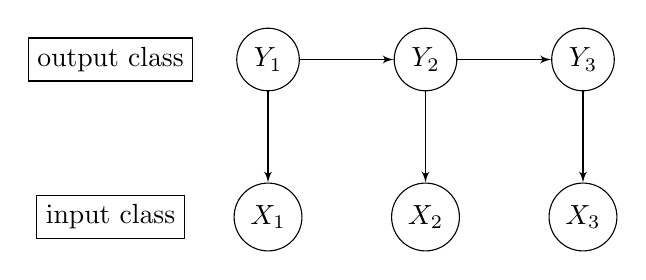
\begin{tikzpicture}
    \tikzset{vertex/.style = {shape=circle,draw,minimum size=1.5em}}
    \tikzset{edge/.style = {->,> = latex'}}
    % vertices
    \node[draw] at (-2, 0) {output class};
    \node[draw] at (-2, -2) {input class};
    \node[vertex] (Y1) at  (0,0) {$Y_1$};
    \node[vertex] (Y2) at  (2,0) {$Y_2$};
    \node[vertex] (Y3) at  (4,0) {$Y_3$};
    \node[vertex] (X1) at  (0,-2) {$X_1$};
    \node[vertex] (X2) at (2,-2) {$X_2$};
    \node[vertex] (X3) at (4,-2) {$X_3$};
    %edges
    \draw[edge] (Y1) to (Y2);
    \draw[edge] (Y2) to (Y3);
    \draw[edge] (Y1) to (X1);
    \draw[edge] (Y2) to (X2);
    \draw[edge] (Y3) to (X3);
\end{tikzpicture}

Parametrized distributions:
\begin{itemize}
    \item transition $P(Y_t|Y_{t-1}) = Mulitnomial_{Y_{t-1}}$
    \item emission $P(X_t | Y_t) = Gaussian(\mu_y, \sigma_y)$
    \item start $P(Y_1) = Multinomial$ 
    \item joint $P(X_{1:k}, Y_{1:k}) = P(Y_1) \prod_{t=1}^{k} P(X_t | Y_t) \prod_{t > 1}^k P(y_t | y_{t-1})$
\end{itemize}

\subsection{Supervised Learning}
\label{sub:supervised_learning}

\subsubsection{Multinomial Emissions}
\label{ssub:Multinomial Emissions}

Objective:
\begin{equation*}
    argmax_{\pi, \theta, \phi} Pr(y_{1 \ldots t}, x_{1 \ldots t} | \pi, \theta, \phi)
\end{equation*}
For $y \in \{c_1, c_2\}, x \in \{v_1, v_2\}$, maximum likelihood:
\begin{align*}
    \pi_{c_1^{\text{start}}} &= \# c_1^{\text{start}} / (c_1^{\text{start}} + c_2^{\text{start}}) \\
    \theta_{c1|c1} &= \#(c_1, c_1) / (\#(c_1, c_1) + \#(c_2, c_1)) \\
    \theta_{c1|c2} &= \#(c_1, c_2) / (\#(c_1, c_2) + \#(c_2, c_2)) \\
    \phi_{v1|c1} &= \#(v_1, c_1) / (\#(v_1, c_1) + \#(v_2, c_1)) \\
    \phi_{v1|c2} &= \#(v_1, c_2) / (\#(v_1, c_2) + \#(v_2, c_2)) \\
\end{align*}

\subsubsection{Gaussian Emissions}
\label{ssub:Gaussian Emissions}


\begin{align*}
    \pi_{c_1^{\text{start}}} &= \# c_1^{\text{start}} / (c_1^{\text{start}} + c_2^{\text{start}}) \\
    \theta_{c1|c1} &= \#(c_1, c_1) / (\#(c_1, c_1) + \#(c_2, c_1)) \\
    \theta_{c1|c2} &= \#(c_1, c_2) / (\#(c_1, c_2) + \#(c_2, c_2)) \\
    \mu_{c1} &= \text{mean of } c_1 \\
    \mu_{c2} &= \text{mean of } c_2 \\
    \sigma_{c1}^2 &= \frac{1}{\# c_1} \sum_{t | y_t = c_1} (x_t - \mu_{c_1})^2 \\
    \sigma_{c2}^2 &= \frac{1}{\# c_2} \sum_{t | y_t = c_2} (x_t - \mu_{c_2})^2 \\
\end{align*}

\subsubsection{Monitoring and MLE}
\label{ssub:Monitoring and ML}

\textbf{Monitoring}: what is the probability of $y_i = c_1$ at any $i$? \\
iterate $Pr(y_i | x_{1 \ldots i}) \propto Pr(x_i | y_i) \sum_{y_{i-1}} Pr(y_i | y_{i-1}) Pr(y_{i-1} | x_{1 \ldots i-1})$

\medskip

\textbf{Most Likely Explanation}: $argmax_{y_1 \ldots y_t} Pr(y_{1 \ldots t} | x_{1 \ldots t})$? Viterbi algorithm! \\
iterate $\max_{y_{1 \ldots i}} Pr(y_{1 \ldots i+1} | x_{1 \ldots i}) \propto \max_{y_i} Pr(y_{i+1} | y_i) Pr(x_i | y_i) \max_{y_{1 \ldots i-1}} Pr(y_{1 \ldots i} | x_{1 \ldots i-1})$

\begin{ex}{Belief Monitoring and Most Likely Sequence}
    see \href{./cs489-HMM.pdf}{CS489-HMM.pdf}
\end{ex}

\section{Recurrent Neural Networks}
\label{sec:recurrent_neural_networks}

Graphical Model: \\
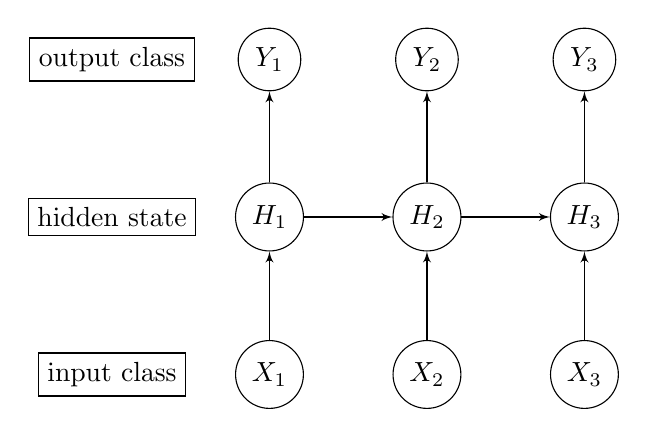
\begin{tikzpicture}
    \tikzset{vertex/.style = {shape=circle,draw,minimum size=1.5em}}
    \tikzset{edge/.style = {->,> = latex'}}
    % vertices
    \node[draw] at (-2, 2) {output class};
    \node[draw] at (-2, 0) {hidden state};
    \node[draw] at (-2, -2) {input class};
    \node[vertex] (Y1) at  (0,2) {$Y_1$};
    \node[vertex] (Y2) at  (2,2) {$Y_2$};
    \node[vertex] (Y3) at  (4,2) {$Y_3$};
    \node[vertex] (H1) at  (0,0) {$H_1$};
    \node[vertex] (H2) at  (2,0) {$H_2$};
    \node[vertex] (H3) at  (4,0) {$H_3$};
    \node[vertex] (X1) at  (0,-2) {$X_1$};
    \node[vertex] (X2) at (2,-2) {$X_2$};
    \node[vertex] (X3) at (4,-2) {$X_3$};
    %edges
    \draw[edge] (H1) to (H2);
    \draw[edge] (H2) to (H3);
    \draw[edge] (H1) to (Y1);
    \draw[edge] (H2) to (Y2);
    \draw[edge] (H3) to (Y3);
    \draw[edge] (X1) to (H1);
    \draw[edge] (X2) to (H2);
    \draw[edge] (X3) to (H3);
\end{tikzpicture}

HMMs have more flexible queries, RNNs have more expressive distributions

\subsection{Belief Monitoring}
\label{sub:Belief Monitoring}

$P(Y_1, X_1) =$
\begin{itemize}
    \item sigmoid or softmax (distribution over binary and categorial outputs)
    \item linear (gaussian distribution with unit variance)
\end{itemize}

\section{Deep Neural Networks}
\label{sec:deep_neural_networks}

\subsection{Overview}
\label{sub:deep_neural_network_overview}

\textbf{Deep Neural Network} ann with many hidden layers
\begin{itemize}
    \item[+] high expressiveness
    \item[-] vanishing gradient
    \item[-] avoiding overfitting
\end{itemize}

Applications:
\begin{itemize}
    \item speech recognition
    \item image recognition: ImageNet (3.07\% by Inception V4)
    \item machine translation
    \item control \ldots
\end{itemize}

\subsection{Vanishing Gradient}
\label{sub:vanishing_gradient}

With sigmoid and hyperbolic activation function, gradient is always $leq$ 1. Therefore, since backprop at each layers multiplies by gradient, the gradient becomes very small as we progress back through layers

\begin{align*}
    \frac{\delta y}{\delta w_4} &= \sigma'(a_4) \sigma(a_3) \\
    \frac{\delta y}{\delta w_3} &= \sigma'(a_4) w_4 \sigma'(a_3) \sigma(a_2) \leq \frac{\delta y}{\delta w_4} 
\end{align*}

Solutions:
\begin{itemize}
    \item pre-training
    \item ReLU $h(a) = \max(0, a)$
        \begin{itemize}
            \item gradient is 0 or 1
            \item sparse computation
            \item softplus $h(a) = \log (1 + e^a)$
        \end{itemize}
    \item Maxout: learn a piecewise activation function that is the max of $k$ linear functions (used with dropout)
        \begin{itemize}
            \item $h_i(x) = \max_{j \in [1, k]} (z_{ij})$ where $z_{ij} = x^T W_{ \ldots ij} + b_{ij}$
            \item doesn't have any places where gradient is close to 0
            \item enhances accuracy of dropout averaging
        \end{itemize}
\end{itemize}

\subsection{Overfitting}
\label{sub:overfitting}

High expressivity increases risk of overfitting

Solutions:
\begin{itemize}
    \item regularization
    \item data augmentation
    \item dropout: randomly drop some units from the network when training
        \begin{itemize}
            \item training: unit $x$ is dropped with prob $p$
            \item testing: multiply output of unit $x$ by $1-p$
            \item approximate form of ensemble learning
        \end{itemize}
\end{itemize}


\section{Convolutional Neural Networks}
\label{sec:convolutional_neural_networks}

\subsection{Convolutions}
\begin{align*}
    \intertext{continuous}
    y(i) &= \int_t x(t) w(i-t) dt \\
         &= (x * w)(t)
    \intertext{discrete}
    y(i) &= \sum_{-\infty}^\infty x(t) w(i-t) dt \\
\end{align*}

\begin{ex}{vertical edge detection}
    \begin{align*}
        y(i, j) &= x(i, j) - x(i -1, j) \\
        w(i - t_1, j - t_2) &= \begin{cases}
            1, &\text{ if } t_1 = i, t_2 = j \\
            -1, &\text{ if } t_1 = i+1, t_2 = j \\
            1, &\text{ otherwise }
        \end{cases}
    \end{align*}
\end{ex}

\subsection{CNN}
\label{sub:cnn}

In neural networks
\begin{description}
    \item[convolution] linear combination of a subset of units based on a specific pattern of weights 
    \item[pooling] commutative math operation combining several units (max, min, average \ldots)
    \item[CNN] network with alternating convolution and pooling, where some convolution weights are shared
\end{description}
\begin{align*}
    a_j &= \sum_i w_{ji} z_i \\
    \intertext{combine with an activation function to produce a feature}
    z_j &= h(\sum_i w_{ji}z_i)
\end{align*}


\medskip

Benefits:
\begin{itemize}
    \item sparse interactions
    \item parameter sharing
    \item locally equivarient
        \begin{itemize}
            \item locally invariant to translation
            \item handle inputs of varying length
        \end{itemize}
\end{itemize}

Applications:
\begin{itemize}
    \item image processing
    \item data with sequential, spatial, or tensor patterns
\end{itemize}

\section{Recurrent and Recursive Neural Networks}
\label{sec:recurrent_and_recursive_neural_networks}

\subsection{Recurrent Neural Network}
\label{sub:recurrent_neural_network}

Output is fed back to the network as inputs, so the network can unroll to handle variable length data

\begin{itemize}
    \item train with BPTT, by unrolling the network a number of steps
    \item weight sharing combines gradients of shared weights into single gradient
    \item challenges
        \begin{itemize}
            \item gradient vanishing and exploding
            \item long range memory
            \item prediction drift
        \end{itemize}
\end{itemize}

Long Short Term Memory (LSTM) networks tackle that challenge by using gates to control memory (input, forget, output)

\subsubsection{Uses}
\label{ssub:Uses}

\begin{itemize}
    \item belief monitoring
        \begin{itemize}
            \item RNN can simulate and generalize HMM
        \end{itemize}
    \item bi-directional RNN
        \begin{itemize}
            \item combine past and future evidence
        \end{itemize}
    \item encoder-decoder
        \begin{itemize}
            \item machine translation
            \item question answering
            \item dialog
        \end{itemize}
\end{itemize}

\subsection{Recursive Neural Network}
\label{sub:recursive_neural_network}

Generalize RNN from chains to trees
\begin{itemize}
    \item weight sharing allows trees to fit variable length data
    \item useful for graphs, e.g. semantic parsing tree
\end{itemize}


\section{Autoencoders}
\label{sec:autoencoders}


\subsection{Overview}
Feed-forward neural network for 
\begin{itemize}
    \item compression
    \item denoising
    \item sparse representation
    \item data generation
\end{itemize}

\begin{align*}
    f(x) &= z \\
    g(z) &= x \\
\end{align*}


\subsection{Linearity}
\label{sub:linearity}

\subsubsection{Linear}
\label{ssub:linear_autoencoder}

$f$ and $g$ are both linear
\begin{itemize}
    \item hidden node is a compressed representation
    \item equivalent to PCA if using euclidean norm (squared loss)
\end{itemize}

\begin{equation*}
    \min_W \frac{1}{2} \sum_n \norm{W_g W_f x_n - x_n}^2_2
\end{equation*}


\subsubsection{Non-Linear}
\label{ssub:non_linear_autoencoder}

$f$ and $g$ are both non-linear
\begin{itemize}
    \item hidden node is a non-linear manifold
\end{itemize}
\begin{equation*}
    \min_W \frac{1}{2} \sum_n \norm{g(f(x_n;W_f); W_g) - x_n}^2_2
\end{equation*}


\subsection{Deep and Sparse}
\label{sub:deep}
In theory, one hidden layer is sufficient to represent any possible compression, but in practise more layers is better.
When there are more hidden nodes than inputs, use regularization to constrain: e.g. sparsity with a penalty term

\begin{align*}
    & \min_W \frac{1}{2} \sum_n \norm{g(f(x_n;W_f); W_g) - x_n}^2_2 + c \delta(f(x_n; W_f)) \\
    & \text{where } \delta(f(x_n; W_f)) = \begin{cases}
    1, &\text{ if } f(x_n;W_f) \not = 0 \\
    0, &\text{ if } f(x_n;W_f) = 0
    \end{cases}
    \intertext{approximate objective is L1 regularization}
    & \min_W \frac{1}{2} \sum_n \norm{g(f(x_n;W_f); W_g) - x_n}^2_2 + c \norm{f(x_n; W_f)}_1 \\
\end{align*}

\subsection{Denoising}
\label{sub:denoising}
Consider $\tilde x$, the noisy version of input $x$. Use autoencoder to compress to true representation and reconstruct without noise

\begin{equation*}
    \min_W \frac{1}{2} \sum_n \norm{g(f(\tilde x_n;W_f); W_g) - x_n}^2_2 + c \norm{f(\tilde x_n; W_f)}_1 \\
\end{equation*}

\subsection{Probabilistic}
\label{sub:probabilistic}
Let $f$ and $g$ represent conditional distributions
\begin{align*}
    f &= Pr(h | x; W_f) \\
    g &= Pr(x | h; W_g)
\end{align*}
by using sigmoid, softmax, or linear units at the hidden and output layers

\subsection{Generative Model}
\label{sub:generative_model}

Sample $h$ from some distribution $Pr(h)$ and use the decoder to sample $x$, $Pr(x | h; W_g)$

\section{Generative Networks}
\label{sec:generative_networks}

\subsection{Overview}
\label{sub:overview}
Design a neural network to generate data
\begin{itemize}
    \item input random noise
    \item output data
\end{itemize}

Types
\begin{itemize}
    \item boltzmann machines
    \item sigmoid belief networks
    \item variational autoencoders
    \item generative adversarial networks
    \item generative moment matching networks
    \item sum-product networks
\end{itemize}


\subsection{Variational Autoencoders}
\label{sub:variational_autoencoders}

\subsubsection{Encoder}
\label{ssub:Encoder}

Train encoder $P(h|x; W_g)$ to approach simple and fixed distribution (e.g. $N(h; 0, I)$)
so that you can set $Pr(h) = N(h; 0, I)$, objective:

\begin{align*}
    & \max_W \sum_n Pr(x_n; W_f, W_g) - c KL(Pr(h|x_n; W_f) || N(h; OI) \\
    & \text{where } KL = \text{Kullback-Liebler divergence}
\end{align*}

\subsubsection{Likelihood}
\label{ssub:Likelihood}

\begin{align*}
    Pr(x_n; W_f, W_g) &= \int_h Pr(x_n|h ; W_g) Pr(h | x_n; W_f) dh
    \intertext{since encoder approaches a normal distribution, force it to be gaussian}
    &= \int_h Pr(x_n|h ; W_g) N(h; \mu_n(x_n; W_f), \sigma_n(x_n;W_f)I) dh
    \intertext{approximate by a single sample}
    &\approx Pr(x_n | h_n; W_g) \\
    & \text{where } h_n ~ N(h; \mu_n(x_n; W_f), \sigma_n(x_n;W_f)I)\end{align*}


\subsection{Generative Adversarial Networks}
\label{sub:generative_adversarial_networks}

\subsubsection{Overview}
\label{ssub:gan_overview}


Two networks:
\begin{enumerate}
    \item generator $g(z; W_g) \to x$
    \item discriminator $d(x;W_d) \to Pr(x \text{ is real})$
\end{enumerate}

Objective
\begin{equation*}
    \min_{W_g} \max_{W_d} \sum_n \log d(x_n; W_d) + \log(1- d(g(z_n;W_g); W_d))
\end{equation*}

Issues
\begin{itemize}
    \item one network may dominate the other
    \item local convergence
\end{itemize}

\subsubsection{Training}
\label{ssub:gan_training}

\begin{algorithmic}
    \For{$k$ steps}
    \State sample $z_1 \ldots z_m$ from $Pr(z)$
    \State sample $x_1 \ldots x_m$ from training set
    \State update discriminator with SGD
    \begin{equation*}
        \nabla W_d (\frac{1}{m} \sum_{n=1}^m [\log d(x_n; W_d) + \log(1- d(g(z_n;W_g); W_d))])
    \end{equation*}
    \EndFor
    \State sample $z_1 \ldots z_m$ from $Pr(z)$
    \State update generator with SGD
    \begin{equation*}
        \nabla W_g (\frac{1}{m} \sum_{n=1}^m \log(1- d(g(z_n;W_g); W_d)))
    \end{equation*}
\end{algorithmic}

In the limit, yields
\begin{itemize}
    \item $Pr(x|z;W_g) \to $ true data distribution
    \item $Pr(x \text{ is real}; W_d) \to 0.5$, real and fake data are indistinguishable
\end{itemize}

\section{Ensemble Learning}
\label{sec:ensemble_learning}

\subsection{Overview}
\label{sub:ensemble_overview}
\textbf{ensemble learning} method to select and combine ensemble of hypotheses into a better hypothesis, can enlarge hypothesis space


\subsection{Bagging}
\label{sub:bagging}
\textbf{bagging} majority voting
\begin{itemize}
    \item each $h_i$ is wrong with probability $p$
    \item the majority of $k$ is wrong with probability $\sum_{k > n/2} \binom{n}{k} p^k (1-p)^{n-k}$
\end{itemize}
weighted majority
\begin{itemize}
    \item give weight proportional to hypothesis accuracy
\end{itemize}

\subsection{Boosting}
\label{sub:boosting}
\begin{description}
    \item[boosting] learn with a weighted training set (more weight = more important) and increase the weight on examples that are misclassified, this can \textit{boost} a weak learner
    \item[weak learner] produces hypothesis at leas as good as random classifier
\end{description}

Applications
\begin{itemize}
    \item sensor fusion
    \item collaborative filtering (Netflix challenge)
    \item body part recognition (kinect)
\end{itemize}

\subsubsection{Framework}
\label{ssub:Framework}

\begin{algorithmic}
    \State set all instance weights $w_x = 1$    
    \Repeat
    \State $h_i \gets$ learn(dataset, weights)
    \State increase $w_x$ of misclassified examples $x$
    \Until{sufficient number of hypotheses} \\
    \Return weighted majority of $h_i$s with weights $w_i$ proportional to accuracy of $h_i$
\end{algorithmic}

\subsubsection{Paradigm}
\label{ssub:Paradigm}

\begin{itemize}
    \item don't try to learn perfect hypothesis, just learn simple rules of thumb and boost them
    \item good generalization
    \item principled approach to combine many hypotheses
\end{itemize}

\subsubsection{AdaBoost}
\label{ssub:AdaBoost}

\begin{algorithmic}
    \State $w_j \gets 1/N \ \forall j $
    \For{$m=1 \to M$}
    \State $h_m \gets$ learn(datset, $w$)
    \State $err \gets 0$
    \For{each $(x_j, y_j)$ in dataset}
    \If{$h_m(x_j) \not = y_j$}
    \State $err \gets err +w_j$
    \EndIf
    \EndFor
    \For{each $(x_j, y_j)$ in dataset}
    \If{$h_m(x_j) = y_j$}
    \State $w_j \gets w_j \frac{err}{1-err}$
    \EndIf
    \EndFor
    \State $w \gets \text{ normalize}(w)$
    \State $z_m \gets \log (\frac{1-err}{err})$
    \EndFor \\
    \Return $weighted-majority(h,z)$
\end{algorithmic}

\section{Bagging and Distributed Computing}
\label{sec:bagging_and_distributed_computing}

\subsection{Independent Bagging}
\label{sub:independengt_bagging}
\begin{description}
    \item[bagging] combine independent classifiers that were trained on subsets of the dataset (sampling w/o replacement)
    \item[bootrap sampling] sample subset of data
    \item[random projection] sample subset of features
    \item[random forest] bag of decision trees
\end{description}

\begin{algorithmic}
    \For{$k=1 \to K$}
    \State $D_k \gets$ sample data subset
    \State $F_k \gets$ sample feature subset
    \State $h_k \gets$ train classifier based on $D_k$ and $F_k$
    \EndFor
    \If{classification} \\
    \Return $majority(h_1(x) \ldots h_K(x))$
    \ElsIf{regression} \\
    \Return $average(h_1(x) \ldots h_K(x))$
    \EndIf
\end{algorithmic}

Kinect: body part recognition
\begin{itemize}
    \item infrared + gray-scale depth map
    \item features: depth difference between pairs of pixels
    \item classification: forest of decision trees
\end{itemize}

\subsection{Distributed Computation}
\label{sub:distributed_computation}
``big data'' aka large scale machine learning requires distributed computation
\begin{itemize}
    \item GPU: performing arithmetic operations on all elements of a tensor in parallel
    \item CPU: train classifiers with a different subset on each core
        \begin{itemize}
            \item don't combine parameters (e.g. adding together two NN that encode xor doesn't encode xor)
            \item combine \textit{predictions} not parameters
        \end{itemize}
\end{itemize}

\section{Stream Learning}
\label{sec:stream_learning}

\subsection{Overview}
\label{sub:stream_learning_overview}

\begin{description}
    \item[online learning] new data continuously arrives
    \item[stream learning] train as new data arrives
\end{description}

challenges
\begin{itemize}
    \item can't store all the data, revisit older data
    \item algorithm must keep up with the stream, process quickly
    \item patterns may change over time, must be able to update hypothesis on every point or batch
\end{itemize}

\subsection{Algorithms}
\label{sub:algorithms}

\begin{itemize}
    \item bayesian learning: lends itself naturally because bayes theorem updates on every example given current state
    \item optimization-based learning: objective
\end{itemize}

\begin{alignat*}{3}
    & argmin_\theta \sum_n Loss(x_n, y_n; \theta) \\
    & \text{where } Loss \text{ could be} &&= - \log Pr(y|x;\theta) \text{ neg log likelihood} \\
    & &&= [y - h_\theta (x)]^2 \text{ squared error}
\end{alignat*}

\subsection{Gradient Descent}
\label{sub:gradient_descent}

Gradient Descent
\begin{align*}
    \theta^{(i+1)} & \gets \theta^{(i)} - \alpha_i \sum_n \nabla Loss(x_n, y_n; \theta^{(i)}) \\
    \text{where } & \alpha \in [0,1] \text{ is the learning rate} \\
    &n \text{ indexes data points} \\
    &m \text{ indexes GD iterations}
\end{align*}

Stochastic Gradient Descent
\begin{align*}
    \theta^{(n+1)} & \gets \theta^{(n)} - \alpha_n \sum_n \nabla Loss(x_n, y_n; \theta^{(n)}) \\
    \text{where } & n \text{ indexes data points and iterations} \\
\end{align*}

Converge if $\sum_{n=1}^\infty \alpha_n = \infty$ and $\sum_{n=1}^\infty (\alpha_n)^2 < \infty$

Adagrad: use a different step size for each parameter
\begin{align*}
    \theta^{(n+1)} & \gets \theta^{(n)} - \frac{\alpha_n}{\tau + \sqrt{s_m^{(n)}}} (\frac{\partial Loss(x_n, y_n; \theta^{(n)})}{\partial \theta_m^{(n)}})^2 \\
    \text{where } & n \text{ indexes data points and iterations} \\
\end{align*}


\end{document}
